%
% Apunte de Sistemas Operativos
% Copyright (C) 2014 Esteban De La Fuente Rubio (esteban[at]delaf.cl)
%
% Permission is granted to copy, distribute and/or modify this document
% under the terms of the GNU Free Documentation License, Version 1.3
% or any later version published by the Free Software Foundation;
% with no Invariant Sections, no Front-Cover Texts, and no Back-Cover Texts.
% A copy of the license is included in the section entitled "GNU
% Free Documentation License".
%
% Link: http://www.gnu.org/copyleft/fdl.html
%

% MEMORIA PRINCIPAL
\chapter{Memoria principal}
\label{memoria_principal}
Todo programa que se quiera ejecutar dentro del sistema, o sea convertirse en un proceso, requerirá como mínimo dos recursos, utilizar la CPU para ejecutar su código y utilizar memoria RAM para almacenar su código y datos. El primer tema fue discutido en el capítulo \ref{planificacion_monoprocesadores}, la asignación de RAM será discutida en este capítulo donde se abordarán los dos temas principales de administración de memoria principal, correspondientes a direcciones virtuales y memoria virtual.

Es importante recalcar que todo proceso que quiera pasar por la CPU requiere estar cargado en memoria principal. Esto implicará que al inicio del proceso el programa debe ser llevado desde el disco (almacenamiento secundario) a la RAM (memoria principal). Adicionalmente es importante recordar las velocidades de operación de los tipos de almacenamientos existentes y sus capacidades se verán afectadas dependiendo de si se trata de discos, ram, cache o registros de cpu, ver figura \ref{fig:memchart}.

\begin{figure}[htbp]
\centering
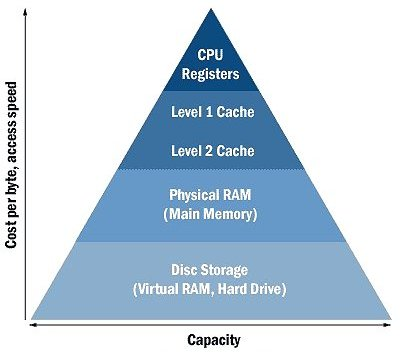
\includegraphics[scale=0.7]{img/C07_memoria/memchart.jpg}
\caption{Tipos de memorias (tiempos, tamaños y costos)}
\label{fig:memchart}
\end{figure}

Finalmente se deberán considerar aspectos relacionados con la protección de la
memoria principal, donde el sistema operativo deberá garantizar que solo los
procesos legítimos puedan hacer uso de cierto espacio de direcciones, evitando
que cualquiera pudiese leer o escribir en cualquier área de la memoria.

\section{Espacio de direcciones}
Originalmente en los ``sistemas operativos'' la administración de la memoria era
bastante simple ya que al existir un solo proceso ejecutándose al mismo tiempo
este se podía copiar completamente a la memoria principal y acceder a los
registros de la misma de forma directa. Sin embargo lo interesante es ver lo que
ocurre en un sistema que utiliza multiprogramación, donde pueden existir
diversos procesos residentes en memoria principal y a todos se les debe asignar
un espacio de memoria para poder ser ejecutados.

La forma más simple de asignar la memoria a diversos procesos es simplemente
tomar todo el programa existente en disco y copiarlo como un solo bloque a la
memoria principal, en cuyo caso para determinar donde se encuentra el proceso
guardado en la memoria basta conocer la dirección inicial, llamada
\textbf{base}, y el tamaño del bloque, llamado \textbf{límite}, en la figura
\ref{fig:baselimite} tenemos una $base=300040$ y un $limite=120900$. Para
movernos dentro del bloque del proceso en la memoria utilizamos un
\textit{offset} o \textbf{desplazamiento}, el cual debe dar como resultado
siempre una dirección dentro del bloque que el proceso tiene asignado, de forma
contraria ocurriría un error de protección o \textit{\textbf{segmentation
fault}}, o sea si la dirección es menor a la base o mayor a la base más el
límite ocurrirá un error, ver figura \ref{fig:segmentation_fault}

\begin{figure}[htbp]
\centering
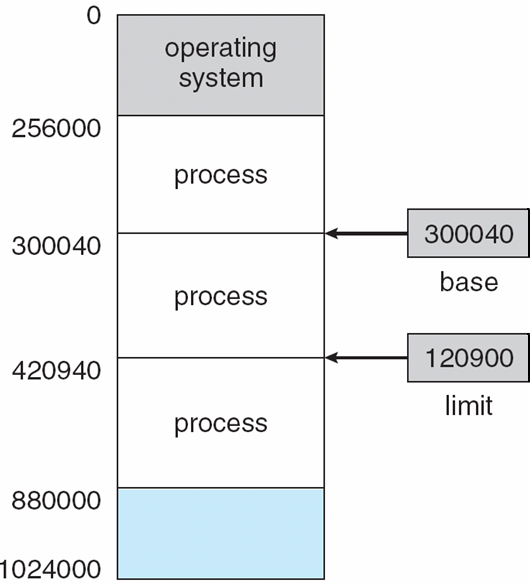
\includegraphics[scale=0.5]{img/C07_memoria/base_limite.png}
\caption{Registro base y límite de un bloque de memoria}
\label{fig:baselimite}
\end{figure}

\begin{figure}[htbp]
\centering
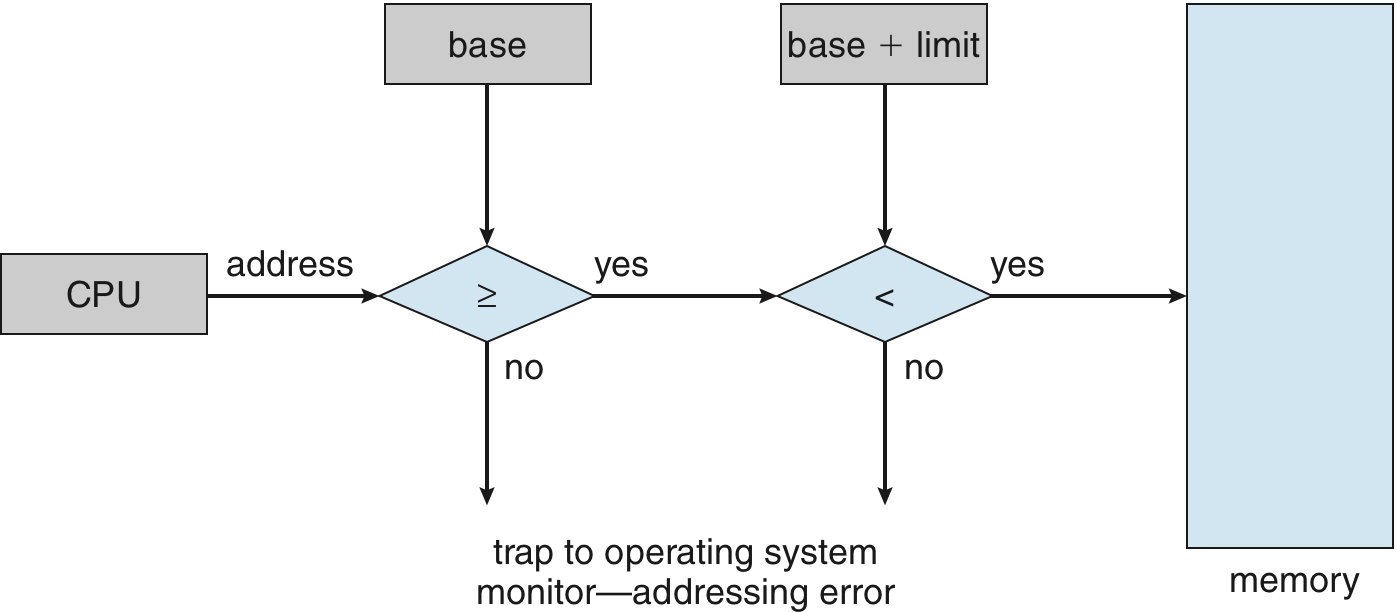
\includegraphics[scale=1]{img/C07_memoria/segmentation_fault.png}
\caption{Protección de memoria, se limita el acceso al bloque del proceso}
\label{fig:segmentation_fault}
\end{figure}

El tipo de asignación descrito anteriormente y mostrado en la figura
\ref{fig:baselimite} corresponde a la \textbf{asignación contigua}, donde todo
el proceso es ubicado en un único bloque de memoria física. De esta forma se
ubicarán diversos procesos en la memoria, pero todos en un único bloque, esto
implica que si no existe espacio contiguo para un proceso deberá sacarse alguno
de los existentes, ver figura \ref{fig:asignacion_contigua}, esto último se
conoce como intercambio y será discutido más adelante.

\begin{figure}[htbp]
\centering
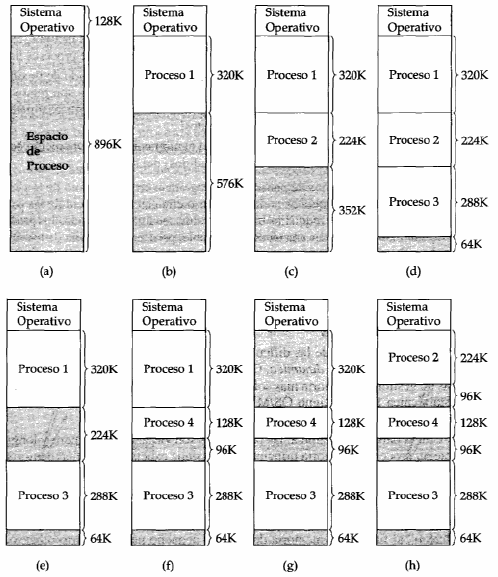
\includegraphics[scale=0.7]{img/C07_memoria/asignacion_contigua.png}
\caption{Asignación contigua}
\label{fig:asignacion_contigua}
\end{figure}

\subsection{Enlace de direcciones}

Una vez se escribe un programa debe ser traducido a código de máquina, ya que el
computador solo entiende direcciones de memoria, no sabe de nombres de variables
ni mucho menos de su semántica. Esto significa que cada una de las variables que
se utilizan dentro del código, y el mismo código, debe ser mapeado a direcciones
de memoria para poder ser utilizado. Lo anterior se conoce como \textbf{enlace
de direcciones} y corresponde al mapeo entre lo que forma el programa (código y
datos) y las direcciones donde se encuentran dichos componentes. Existen
diferentes momentos donde realizar el enlace, cada uno de ellos será mencionado
a continuación y se pueden observar en la figura \ref{fig:memoria_enlaces}.

\begin{figure}[htbp]
\centering
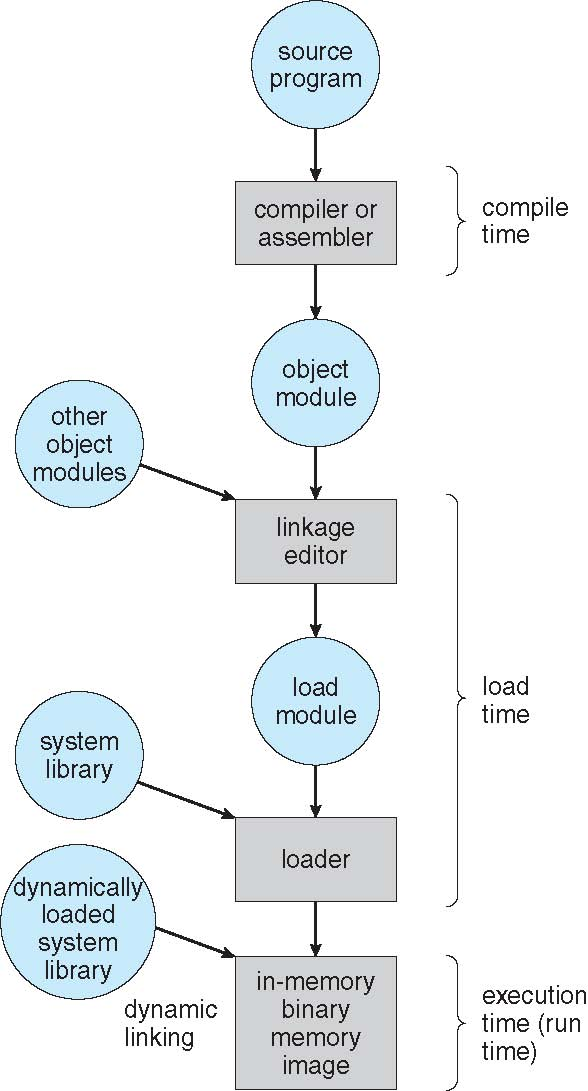
\includegraphics[scale=1]{img/C07_memoria/tipos_enlaces.jpg}
\caption{Tipos de enlaces de direcciones de memoria principal}
\label{fig:memoria_enlaces}
\end{figure}

\subsubsection{Enlace en tiempo de compilación}
Las direcciones de memoria principal son especificadas al momento de compilar el
programa, aquí se indicará donde será cargada cada una de las instrucciones y
variables del código del programa.

Esto tiene diferentes problemas:
\begin{itemize}
	\item El proceso no podrá ser cargado si el bloque que requiere esta
parcialmente o totalmente ocupado.
	\item El proceso no podrá ser movido a otro bloque de memoria una vez
sea cargado.
	\item Se deberán conocer las características físicas de la memoria
principal disponible.
\end{itemize}

Este método tenía sentido en sistemas sin multiprogramación, donde solo un
proceso se encontraba cargado en la ram en todo momento.

\subsubsection{Enlace en tiempo de carga}
En este método el programa generado al compilar no tiene las direcciones de
memoria especificadas, será el sistema operativo el que al cargar el proceso
(estado inicio) asignará las direcciones. De esta forma en diferentes
ejecuciones el programa podría ser ubicado en bloques de memoria diferentes.

El problema aquí seguirá siendo que una vez cargado el programa no podrá ser
movido a otro bloque de memoria. Si por ejemplo se quisiera utilizar intercambio
(al igual que en el caso anterior) el proceso deberá volver al mismo espacio de
direcciones físicas de donde fue sacado, lo cual obviamente representará una
tremenda ineficiencia ya que dicho bloque no podría estar nunca más disponible y
el proceso podría morir de hambruna.

\subsubsection{Enlace en tiempo de ejecución}
En los dos casos anteriores el proceso una vez era cargado en memoria no podía
ser movido a otro bloque, lo que dificultaba que el proceso pudiese crecer (solo
lo haría si hubiesen direcciones contiguas, después de su límite, libres) y
prácticamente imposible hacer intercambio (ya explicado anteriormente).

En este tipo de enlaces el mapeo entre direcciones y los componentes del
programa se realiza en tiempo de ejecución y a medida que el programa va
cambiando (porque necesita crecer o porque es intercambiado) las direcciones de
memoria irán cambiando.

El problema de este método es que la administración de la memoria netamente por
software sería muy complicada y costosa, por las grandes referencias que se
deberían manejar e ir modificando a lo largo de la vida del proceso. Para
solucionar esto y permitir que el enlace pueda ser realizado en tiempo de
ejecución se requiere soporte del hardware, específicamente de la MMU.

\subsection{Direccions virtuales y direcciones físicas}
Uno de los problemas de la multiprogramación es que al existir múltiples
procesos residentes en memoria, si cada proceso utilizará las direcciones de
memoria física para sus enlaces las referencias serían complicadas.

Pensemos por un momento que existe una forma de dividir el programa, de tal
forma que su asignación en memoria no es contigua, el programa se encontraría
dividido por toda la memoria principal, sin embargo para ejecutarse necesita un
espacio de direccionamiento contiguo ya que no se puede cortar un bloque de
datos en un punto para luego continuarlo en otra parte de la memoria física.

Otro escenario interesante donde existen problemas es que sucede si necesitamos
ejecutar un programa que requiere más memoria principal de la que disponemos.

Los casos anteriores se simplifican enormemente al utilizar el concepto de
direcciones virtuales y físicas, donde el espacio de direccionamiento virtual
será contiguo para cada proceso, sin embargo el mapeo de dicho espacio virtual
no será necesariamente contiguo en la memoria física.

Adicionalmente, al ser espacio virtual, se podrían tener más direcciones
virtuales que las físicamente soportadas. Esto tendrá sentido más adelante
cuando se vean paginación y segmentación, sin embargo se puede adelantar que un
proceso solo mantendrá cargado lo que necesita y no todo el código o datos del
programa. Esto permitirá cargar programas más grandes que la memoria principal
disponible mediante el uso de direcciones virtuales.

Este mismo concepto es el requerido para el enlace en tiempo de ejecución, donde
un proceso verá el mismo esquema de direcciones virtuales siempre, pero será la
MMU la que se encargará de actualizar las referencias físicas de dichas
direcciones virtuales. Este proceso es totalmente transparente para el proceso y
no se enterará en caso que hayan cambios o lo muevan entre bloques físicos de
memoria.

\subsection{Unidad de administración de memoria MMU}

La unidad de administración (o gestión) de memoria o MMU (del inglés
\textit{Memory Management Unit}) corresponde a la unidad que permite traducir
direcciones virtuales a direcciones reales de memoria principal. De esta forma
un proceso tiene una vista virtual de la memoria, donde varios procesos podrían
tener visión de una misma dirección virtual, la cual es mapeada a direcciones
reales diferentes.

Procesadores de computadores personales iniciales, 8088 o 68000, no contaban con
MMU, por lo cual al no contar con MMU dichas máquinas no podían correr sistemas
operativos Unix (ya que no había fork lo que implica que no hay shell). Esta
característica (MMU) si estaba disponible en los \textit{mainframes} (desde
fines de los 60s). Con los procesadores 386 (Intel) y 68030 (Motorola) estuvo
disponible una MMU en computadores personales a mediados de los 80s.

Sistemas embebidos, como DVD, lavadoras, etc, generalmente no incluyen MMU, ya
que existen menores posibilidades de caídas en el software. En caso que este se
``caiga'' se tiene que reiniciar el sistema, apagándolo, desenchufando o
presionando el botón de encendido por X\footnote{Típicamente 4 segundos.}
segundos.

\section{Asignación no contigua}
A continuación se discutirán métodos de asignación no contigua de la memoria
principal. Recordar que esto aplica a las direcciones físicas, ya que el espacio
de direcciones virtuales siempre será contiguo.

\subsection{Segmentación}
Este tipo de división ya no se utiliza pero es pedagógicamente interesante ya
que es una forma simple de dividir la memoria. Cada proceso necesita al menos 4
segmentos para funcionar, los cuales corresponden al código, los datos, la pila
y el espacio del sistema.

En la figura \ref{fig:memoria} se puede apreciar la división del espacio de
memoria de un proceso, notar que en esta imagen el espacio de datos se encuentra
separado entre las variables globales y el espacio para solicitud dinámica de
memoria (\textit{malloc}). También notar que hay un espacio para bibliotecas
compartidas, de esto se hablará más adelante y tendrá sentido al ver paginación.

\begin{figure}[htbp]
\centering
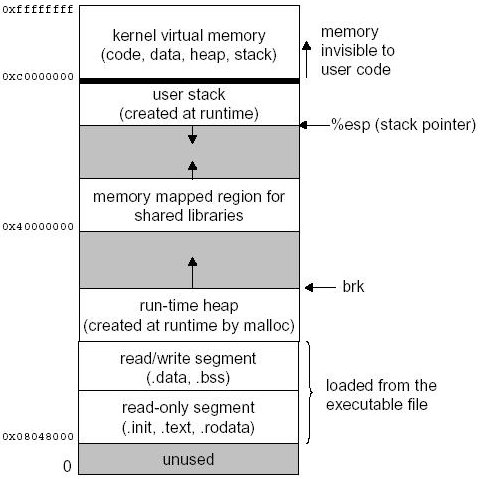
\includegraphics[scale=2]{img/C07_memoria/memoria.png}
\caption{Registro base y límite de un bloque de memoria}
\label{fig:memoria}
\end{figure}

A continuación se describe cada uno de los cuatro segmentos:

\begin{enumerate}[i.]
	\item Código
	\begin{itemize}
		\item Instrucciones binarias del programa.
		\item Solo lectura.
		\item Inicio cercano a la dirección 0, por ejemplo 128 Kb.
	\end{itemize}
	\item Datos
		\begin{itemize}
			\item Variables globales inicializadas.
			\item Variables globales no inicializadas.
			\item heap para malloc y free.
			\item Lectura y escritura.
		\end{itemize}
	\item Pila
	\begin{itemize}
		\item Variables locales.
		\item Información para volver a la rutina que llamo a la
función.
		\item Lectura y escritura.
	\end{itemize}
	\item Sistema
	\begin{itemize}
		\item No se puede leer ni escribir en modo usuario.
		\item Segmento compartido entre todos los procesos.
		\item Inicia en todos los procesos en la misma dirección de
memoria.
	\end{itemize}
\end{enumerate}

Cada uno de los cuatro segmentos será almacenado de forma contigua en la memoria
física, o sea si el programa esta dividido en cuatro segmentos en la memoria
física habrán cuatro segmentos. Se pueden tener los cuatro segmentos separados
en la memoria real, ya que al utilizar direcciones virtuales todo el proceso se
verá continuo en este espacio lógico.

Notar que todos los procesos comparten la memoria correspondiente a la parte de
sistema (núcleo), sin embargo solo pueden acceder a ella en modo sistema, no en
modo usuario.

Entre la pila y el sistema se encuentra una zona de espacio de memoria no
asignada utilizada para crecer al ir solicitando más memoria con
sbrk\footnote{man sbrk}. Por razones históricas existe el \textit{segmentation
fault}, sin embargo actualmente debiese ser \textit{page fault}.

El sistema real, la máquina, tendrá una cierta cantidad de memoria física, por
ejemplo 4 Mb, entonces un proceso verá sus direcciones virtuales (descritas
anteriormente) mapeadas a las direcciones reales en la memoria física
disponible.

La traducción de direcciones virtuales a reales será realizada mediante la tabla
de segmentos, donde existe una tabla por cada proceso (que pertenece a su
contexto). Dependiendo de la implementación de la tabla de segmentos se pueden
guardar diferentes registros (direcciones) todas apuntando a poder obtener la
dirección física en memoria principal a partir de una dirección virtual.

En la figura \ref{fig:tabla_segmentos} se puede observar el proceso de
traducción de una dirección virtual utilizando segmentos a una dirección física.
Importante mencionar que la dirección lógica entregará el segmento al que
corresponde y un desplazamiento dentro de dicho segmento. De esta forma
podríamos tener una dirección lógica dentro del segmento de datos y otra dentro
de la pila, ambas con el mismo desplazamiento. Una vez se tiene el segmento se
busca en la tabla de segmentos si dicho segmento tiene asociada una dirección
base (física) asignada, si lo tiene se suma a su desplazamiento (previa
verificación que este dentro del límite del segmento) y se obtiene la dirección
real en la memoria secundaria.

\begin{figure}[htbp]
\centering
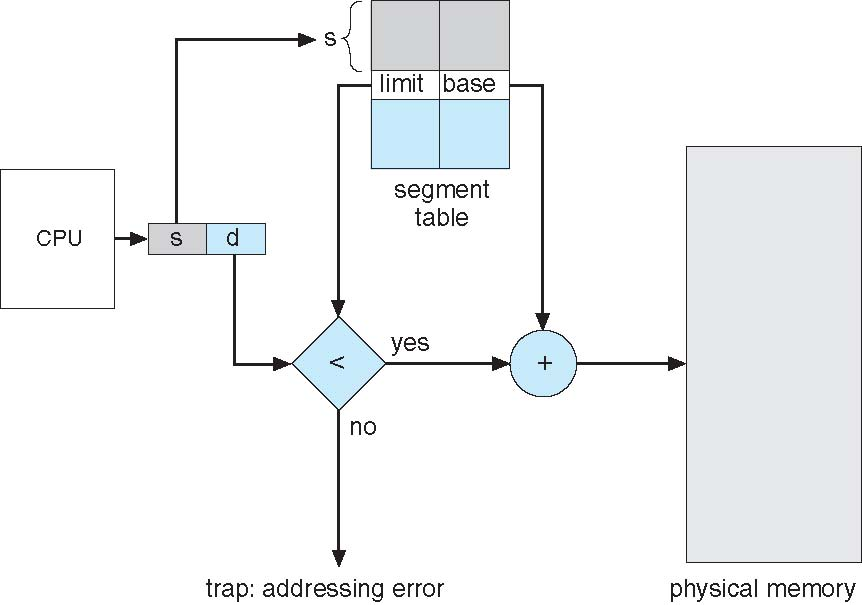
\includegraphics[scale=1]{img/C07_memoria/tabla_segmentos.jpg}
\caption{Traducción de segmentos}
\label{fig:tabla_segmentos}
\end{figure}

Esta traducción se realiza por hardware en la MMU, lo cual toma aproximadamente
un ciclo del reloj. La MMU mantiene la tabla del proceso en ejecución solamente,
ya que sería costoso (para el hardware) mantener todas las tablas.

Al existir un cambio de contexto la tabla de segmentos se almacena en el
descriptor del proceso y se debe cambiar la tabla del proceso saliente por la
del proceso entrante.

\subsubsection{Administración de segmentos}

Se deben crear tres segmentos al crear un proceso (fork), al hacer exec o al
hacer sbrk, importante recordar que el segmento de sistema no se crea en la
memoria principal, ya que dicho segmento es compartido entre todos los sistemas
y corresponde el código y datos del sistema operativo. La destrucción de los
segmentos se realiza cuando el proceso termina.

El núcleo mantiene un \textit{heap} de memoria para segmentos, el cual es
utilizado para los segmentos que se van creando y destruyendo. Esta se
administra de forma similar a como se maneja malloc y free.

Por ejemplo para la administración de los segmentos se puede utilizar una lista
enlazada de pedazos de segmentos disponibles. Esta lista representa trozos de
memoria contigua, en la cual cuando se crea un segmento se debe buscar cual es
el ``mejor'' pedazo para ubicar el segmento del proceso. Cuando se destruye un
segmento se debe devolver a esta lista el espacio liberado, y de ser necesario
unirlo a un segmento contiguo que ya estuviese libre.

El mayor problema es el elegir que segmento entregar, ya que se debe considerar
el tamaño del mismo. Históricamente existen 3 estrategias:

\begin{itemize}
	\item \textbf{First-fit o primer ajuste}: recorrer secuencialmente la
lista desde el inicio hasta encontrar un espacio que alcance para el segmento,
se divide el segmento usando el tamaño preciso y devolviendo lo que no se
ocupará a la lista enlazada. Esto achica trozos disponibles dejando cada vez
tamaños más pequeños libres.
	\item \textbf{Best-fit o mejor ajuste}: busca en toda la lista cual es
el tamaño más cercano  suficiente para el segmento. El problema es que debe
recorrer toda la lista y va dejando pedazos demasiado pequeños cada vez.
	\item \textbf{Worse-fit o peor ajuste}: busca en toda la lista y entrega
el peor caso, es teórico y no se usa.
\end{itemize}

De los anteriores el más eficiente es \textit{first-fit}, ya que
\textit{best-fist} deja muchos segmentos pequeños, tan pequeños que no sirven
para ningún segmento. Adicionalmente se debe recorrer la lista completa cada
vez, lo cual no es bueno.

Una mejora a \textit{first-fit}, quedando como el mejor mecanismo para la
asignación, es el uso de una lista circular. De esta forma no se parte cada vez
del inicio de la lista, sino que se parte desde donde se dejo la última vez .
Esto evita que los pedazos pequeños queden todos al inicio y la búsqueda sea más
rápida, distribuyendo uniformemente los pedazos dentro de la lista.

Las técnicas anteriores producen el problema de \textbf{fragmentación externa},
los métodos anteriores producen pedazos de memoria pequeñas, que no pueden ser
utilizados, sin embargo la suma de estos pedazos pueden servir para atender a un
segmento. Ejemplo, 5 trozos de 1K, se necesita un segmento de 3K, con los 5
trozos no se puede atender al segmento, pero si se pudieran unir si se podría.

Como solución al problema de fragmentación externa existe la
\textbf{compactación}, la cual une los segmentos libres cambiando las
direcciones reales, se deben corregir las tablas de segmentos de los procesos
afectados. Las direcciones virtuales no cambian, por lo cual el proceso de
compactación es transparente para los procesos. El problema de esta solución, es
que se introduce una pausa al momento de ser realizada la compactación por el
tiempo requerido para realizar la copia desde un lado de la memoria principal a
otro, aún así esto es mejor que no poder entregar memoria.

Otra alternativa a la falta de memoria, es el cambio de memoria entre RAM y
disco, mediante el uso de memoria virtual o \textit{swap} lo cual será visto más
adelante.

\subsubsection{Potencial de la segmentación}
Si bien segmentación no es lo que actualmente se utiliza, tiene la ventaja de
ser más sencillo y fácil de implementar.

\begin{enumerate}[i.]

\item \textbf{Incremento del espacio para \textit{heap}.}

Supongamos tenemos un área de datos en un proceso, donde se encuentra su heap.
malloc pide memoria pero no hay, por lo cual es llamado sbrk para aumentar el
tamaño del segmento de datos.

Para implementar la llama a sistema sbrk el núcleo debe:
\begin{enumerate}
	\item Solicitar un segmento más grande.
	\item Copiar el contenido.
	\item Liberar el antiguo segmento.
	\item Actualizar la tabla de segmentos.
\end{enumerate}

Lo que el proceso ve es lo ``mismo'', solo cambia el límite virtual del
segmento, lo cual es natural ya que el proceso está pidiendo memoria. Sin
embargo los cambios de direcciones reales del segmento, lo cual si cambio, no es
visible por el proceso.

Se puede utilizar una optimización que no copie, realloc permite hacer esto
extendiendo el segmento a un trozo contiguo libre. De hecho malloc
automáticamente utilizará sbrk o realloc dependiendo de la situación, sin
embargo si no hay un segmento contiguo libre necesariamente se debe copiar hacia
otro lado ya que en segmentación cada segmento se debe encontrar de forma
contigua en la memoria física.

\item \textbf{Desborde de la pila}

Esto ocurre automáticamente al ir llamando funciones (por ejemplo de forma
recursiva). Para evitar que se produzca un \textit{overflow}, el núcleo pide más
memoria de forma transparente para el proceso más memoria. Esto se hará
adivinando cuando se podría requerir más memoria para la pila, y el núcleo
interrumpirá al proceso (sin que este se entere) y la aumentará.

En caso que ocurriese un desborde de la pila y se tratase de acceder a un área
que no ha sido asignada ocurrirá un \textit{segmentation fault}. Donde si el
proceso no atrapa la señal del \textit{segmentation fault}, el núcleo enviará
una señal al proceso padre indicando el error y será el padre (la shell) quien
imprimirá el mensaje.

\item \textbf{Implementación de fork}

\begin{verbatim}
int pid = fork();
if (pid==0) {
  // hijo
} else {
  // padre
}
\end{verbatim}

Como el segmento de código es de solo lectura y común para todos los hijos, se
puede mapear para todos los hijos el mismo trozo físico en la memoria real para
dicho segmento. Esto evita tener que copiar el código y ahorra memoria
principal.

Si un proceso hace fork y hay una variable global que es modificada por el hijo,
el padre no verá este cambio, ya que los procesos no comparten memoria o sea son
procesos pesados. Cada proceso tendrá su propio segmento de datos.

\item \textbf{Swapping}

Cuando la memoria escasea el scheduler de mediano plazo lleva procesos completos
a disco. El estado del proceso cambia a SWAPPED y se guardan copias al bit de
los segmentos que se envían a disco. En algún momento se llevarán a disco otros
procesos y se restaurará este, lo más probable en otra dirección física de
memoria, esto sigue siendo transparente para el proceso.

Esto es crítico en procesos interactivos. Sigue siendo mejor a no tener memoria
y no poder atender a nuevos o tener que matar procesos. Se trata de evitar
llevar procesos interactivos a disco.

\end{enumerate}

\subsection{Paginación}
La paginación corresponde a otro método de asignación de memoria física no
contigua, el cual es el actualmente utilizado. Básicamente es muy similar a la
segmentación, sin embargo aquí la memoria no se divide por segmentos si no que
se divide en páginas.

Específicamente es el proceso el que se divide en páginas de igual tamaño cada
una de ellas y la memoria principal se divide en marcos de igual tamaño que las
páginas. De esta forma cuando se crea un proceso y se copia el código más los
datos estos son llevados a marcos en la memoria principal los cuales no
necesariamente estarán contiguos. Al igual que en segmentación, desde el punto
de vista de direcciones lógicas las páginas están contiguas.

La paginación no presenta el problema de fragmentación externa, por lo cual no
requiere compactación. Sin embargo el problema que aparece es el de la
\textbf{fragmentación interna}, ya que los marcos al ser de tamaño fijo puede
ocurrir que una página de un proceso no complete el marco quedando espacio libre
dentro de dicho marco. Este espacio puede ser utilizado para crecer
eventualmente, pero de no ser utilizado será desperdiciado.

En la figura \ref{fig:paginacion_varios_procesos} se puede observar como tres
procesos han sido divididos en páginas del mismo tamaño, la memoria principal ha
sido dividida en marcos del mismo tamaño que las páginas. Cada página se ubica
en un marco dentro de la memoria principal. Es la tabla de páginas la que dice
que página se encuentra en que marco.

\begin{figure}[htbp]
\centering
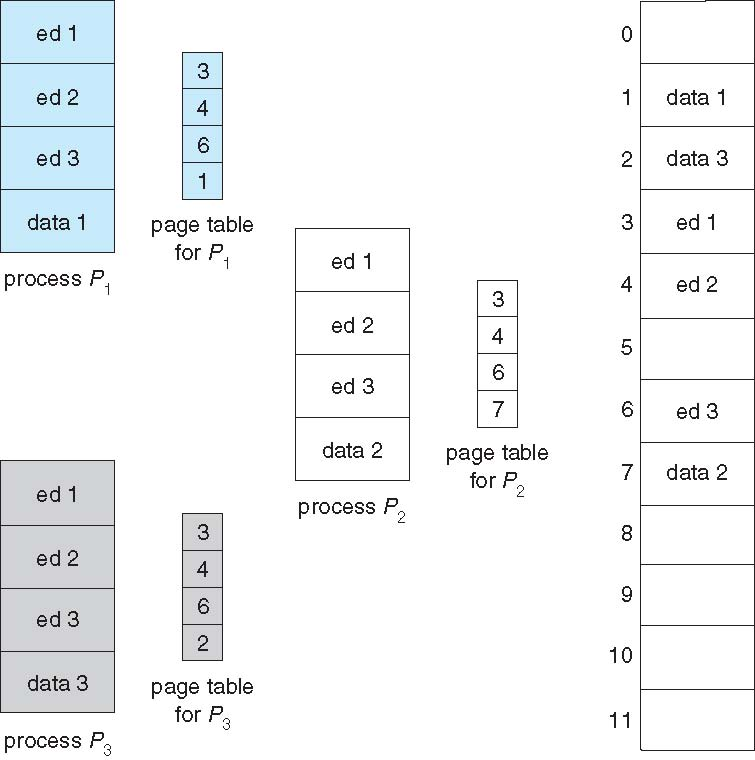
\includegraphics[scale=1]{img/C07_memoria/paginacion_varios_procesos.jpg}
\caption{Ejemplo de paginación con 3 procesos}
\label{fig:paginacion_varios_procesos}
\end{figure}

\subsubsection{Carga dinámica}
El hecho de tener ahora páginas permitirá llevar a la memoria principal partes
del código o datos del programa, no teniendo que llevar todo el código (como
ocurría con segmentación) de esta forma se cargarán bajo demanda las páginas del
proceso y si existen algunas que nunca se lleguen a utilizar entonces nunca
serán cargadas en la memoria principal.

Esto lo que busca es reducir el espacio, específicamente marcos, utilizados por
un proceso en la memoria principal, cargando solo lo que es necesario.

Para utilizar la carga dinámica el sistema operativo deberá vaciar la memoria
cache L1 (de nivel 1) para que se produzcan los fallos de página del proceso que
está en ejecución cada vez que ocurra un cambio de contexto. La acción de vaciar
la caché es la que finalmente representa gran parte del costo del cambio de
contexto.

\subsubsection{Enlace de bibliotecas}
Cuando un programa requiere hacer uso de alguna biblioteca que esta en el
sistema existen dos alternativas para el enlace de las mismas, un enlace
estático y otro dinámico.

En el \textbf{enlace estático} las bibliotecas son agregadas al ejecutable al
momento de la compilación. Esto implica un mayor tamaño en el programa
resultante y eventualmente una mayor cantidad de páginas que cargar en memoria
cuando el programa se ejecute. Esto tiene además el problema que se repetirán
páginas de la biblioteca entre varios procesos que la usen y la tengan enlazada
de forma estática en su código.

En el \textbf{enlace dinámico} al momento de compilar solo se deja una
referencia a las bibliotecas, las cuales deberán ser cargadas por el sistema al
momento de la ejecución del programa pero en un espacio diferente al código del
programa. De esta forma se podrán compartir varias bibliotecas entre varios
procesos en ejecución, en el fondo se compartirán las páginas cargadas
correspondientes a dichas bibliotecas. Si la página requerida no esta cargada
cuando la solicita un proceso P1 se cargará en un marco M1, cuando un proceso P2
requiera la misma página de la biblioteca no se volverá a cargar si no que se
hará referencia al marco M1 ya cargado. Este espacio para cargar bibliotecas
compartidos puede apreciarse en la figura \ref{fig:biblioteca_compartida}.

\begin{figure}[htbp]
\centering
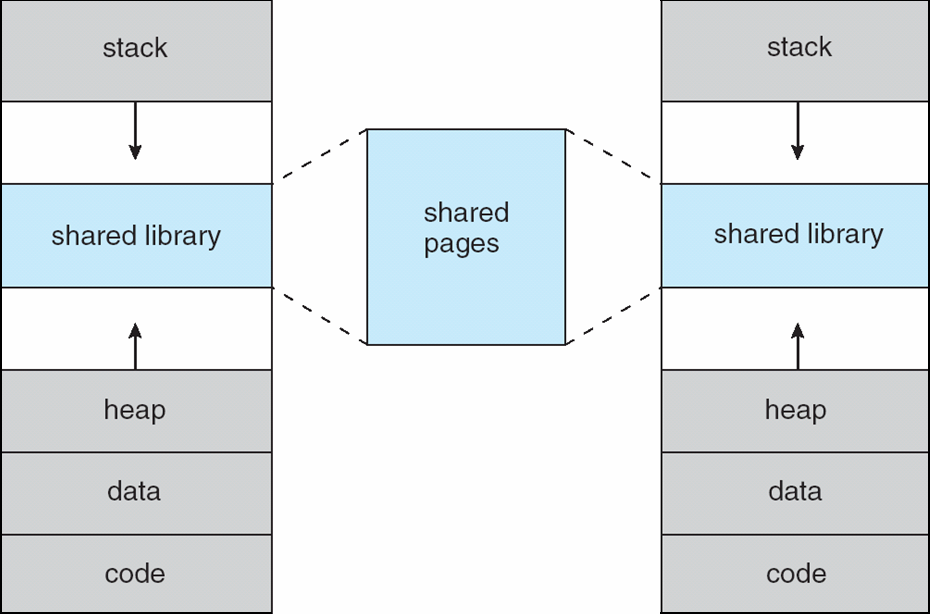
\includegraphics[scale=0.45]{img/C07_memoria/biblioteca_compartida.png}
\caption{Biblioteca compartida entre dos procesos}
\label{fig:biblioteca_compartida}
\end{figure}

Uno de los problemas con el enlace de bibliotecas de forma dinámica es el uso de
variables globales en las bibliotecas. Por lo cual si se esta desarrollando un
software con múltiples hebras no se deberán utilizar bibliotecas que no se han
desarrollado para ser utilizadas en procesos ligeros, ya que pueden aparecer
problemas de \textit{dataraces}.

\subsubsection{Procesos semi-pesados}

Adicionalmente a la idea de bibliotecas compartidas, se pueden tener áreas de
datos compartidas entre procesos. Hasta ahora se habían visto procesos livianos
y procesos pesados. Un proceso semi-pesado corresponde a un proceso que puede
compartir ciertas áreas de memoria con otro proceso.

Supongamos un proceso pesado con Código (C), Datos (D) y Pila (P). Un proceso
semi-pesado podría corresponder al proceso pesado anterior (C, D y P) más un
área para datos (D') que es compartida con otros procesos.

Existen funciones que permiten retornar puntos a espacios de memoria compartida,
como por ejemplo \textit{mmap}.

\subsubsection{Implementación tabla de páginas}

Las tablas de páginas son considerablemente más grandes comparadas con las
tablas de segmentos, esto ya que un programa al ser dividido en páginas por lo
general contendrá más páginas que si fuese dividido en segmentos. Por lo
anterior las tablas de páginas no pueden ser almacenadas completamente en la
MMU, y deben ser mantenidas en la memoria principal.

La situación explicada anteriormente implica que por cada acceso ``útil'' a la
memoria principal se requiere un acceso para buscar la tabla de páginas (para
saber donde está lo solicitado) y otro para acceder a lo solicitado. Este doble
acceso para llegar a la memoria principal significa tiempos mayores de acceso a
los datos requeridos.

Como solución al problema de doble acceso se utiliza \textit{TLB}
(\textit{translation lookaside buffer}), lo cual es un \textit{buffer} para la
tabla de páginas. Por lo cual cuando se hacen consultas primero se revisa en la
\textit{TLB} por la página solicitada, y solo si no está ahí, se va a la memoria
principal por ella.

\subsubsection{Traducción de páginas}

La traducción de páginas corresponde a un proceso similar al de la traducción de
segmentos, de esta también se encarga la MMU. La dirección lógica en este caso
entregará el número de página del proceso y el desplazamiento dentro de la
página. Por ejemplo en un sistema con direcciones de 32 bits se podrían utilizar
20 bits para la página (y marco) y 12 bits para el desplazamiento.

En la figura \ref{fig:tabla_paginas} se observa el proceso de traducción, donde
una vez obtenida la página y el desplazamiento se busca en la tabla de páginas
el marco correspondiente a dicha página. En caso que la página no estuviese
cargada en un marco en la memoria ocurrirá un fallo de página y la página deberá
ser traída desde el disco, si la página no existe o el desplazamiento esta fuera
de rango se produce un \textit{segmentation fault}. Una vez se tiene el marco y
se sabe que el desplazamiento es válido se va a la memoria principal con la
dirección física.

\begin{figure}[htbp]
\centering
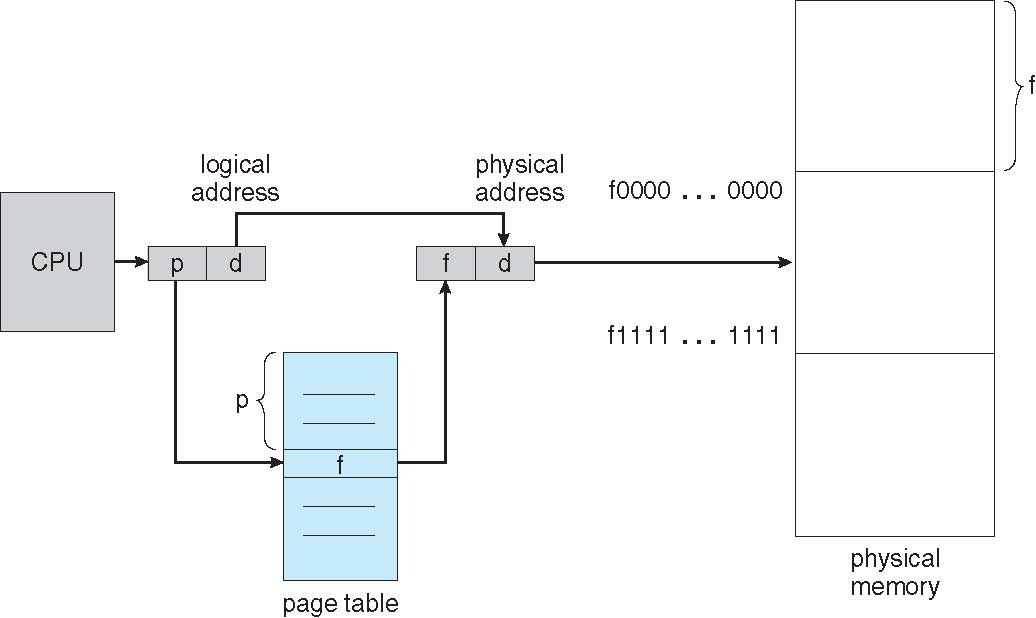
\includegraphics[scale=.9]{img/C07_memoria/tabla_paginas.jpg}
\caption{Traducción de páginas}
\label{fig:tabla_paginas}
\end{figure}

\subsubsection{\textit{Copy on write}}

El objetivo de \textit{copy on write} es hacer un \textit{fork} más eficiente,
donde las páginas serán copiadas en la memoria principal si y solo si son
modificadas. Mientras no sean modificadas las páginas seguirán estando
compartidas entre el padre y el hijo.

En la implementación cuando se realiza \textit{fork} de un proceso las páginas
no son copiadas si no que son marcadas como solo lectura y además se indica que
cuando se quieran escribir primero se deberán copiar. Para esto se utilizarán
campos de los atributos de las páginas para indicar que se debe copiar la página
cuando uno de los procesos (padre o hijo) la desee modificar.

Cada vez que se quiera hacer una modificación se producirá una interrupción que
verificará si la página puede ser escrita, si no lo es se verificará si existe
un bit que indique que se debe copiar, si existe se copiara y luego se
modificará. Si muchos procesos quisieran modificar muchas páginas se producirán
muchas interrupciones, para evitar esto se puede utilizar una heurística que
determine que si se han copiado X páginas a la siguiente interrupción se copien
todas las páginas del proceso a un nuevo espacio, asumiendo que seguirán
ocurriendo interrupciones.

Este método también es conocido como duplicación perezosa de las páginas o copia
bajo demanda.

\subsubsection{Tablas de páginas de dos niveles}

Estos ejemplos son para x86 (32 bits), para procesadores de 64 bits existen
tablas de páginas de 3 niveles asociadas con procesadores de 64 bits.

Para el caso de 32 bits, la dirección de memoria virtual se dividirá en 2
partes. Donde la primera parte a su vez se divide en un bloque \textit{b} (10
bits) y página \textit{p} (10 bits). La segunda parte es el desplazamiento
\textit{d} (12 bits).

En 32 bits el tamaño máximo de memoria que se puede direccionar son 4G, en este
caso la memoria es dividida en 1024 bloques, entonces cada bloque es de 4M. Y
cada bloque es dividido en 1024 páginas, entonces cada página es de 4K.

Existe un directorio de bloques que indica para cada bloque:

\begin{itemize}
	\item \textbf{b}: el bloque.
	\item \textbf{t}: utilizado para entregar la dirección de una tabla de
páginas asociada al bloque \textit{b} (dirección de 10 bits).
	\item \textbf{Atributos}: similares a los de las páginas, pero valido
para todo el bloque (o sea para todas las páginas).
\end{itemize}

Con lo anterior se construye una nueva dirección, formada por $t+p$, que entrega
un puntero directo a la entrada en la tabla de página \textit{t} del bloque
\textit{b}. Con este puntero a la entrada y \textit{p} se puede construir la
dirección real de la página, ya que la entrada de la tabla de páginas (apuntada
por \textit{t}) contiene el marco \textit{m} al cual se le suma \textit{d},
obteniendo la dirección física.

La idea de usar estas dos tablas (por eso se llama tabla de páginas en dos
niveles), es que la mayoría de los procesos requieren menos de 4M. Donde un
proceso ocupará 1 bloque para su código y datos y otro bloque para la pila.
Todas los otros bloques se encontrarán inválidos (no asignados). El espacio que
queda en el bloque es dejado para crecimiento futuro.

El sobre-costo para un típico proceso (menor a 4M) es:
\begin{itemize}
	\item Una tabla para código más datos.
	\item Una tabla para la pila.
	\item Un directorio para manejar los bloques.
\end{itemize}

Tanto el directorio como la tabla de páginas requieren (cada una) 4K, ya que
cada entrada ocupa 32 bits. Por lo cual un proceso menor a 4M requerirá 12K para
manejar su memoria principal. Sobre-costo es muy bajo, menor al 1\% (lo que se
requiere \textit{versus} lo que se podrá direccionar).

Cuando se requiere más memoria, llamando a \textit{sbrk}, se entregarán páginas
dentro del mismo bloque de memoria ya asignado, una vez el bloque se llena se
van pidiendo nuevos bloques de memoria.

Cuando los datos llegan a la dirección de la pila, significa que no hay más
espacio que asignar y \textit{malloc} retornará \textit{NULL} y el proceso no
podrá continuar, asumiendo que terminará cuando \textit{malloc} retorne
\textit{NULL}.

\subsubsection{Tablas de páginas de tres niveles}

Los directorios se referencian de a 4G (o sea se agregan 10 bits más a la
dirección virtual), donde existe otra tabla (tercer nivel) que administra estos
directorios.

En sistemas de 64 bits, se dispone de 64 bits para la dirección, sin embargo
direcciones de 64 bits permitirían referenciar mucha más memoria de la que
actualmente se encuentra disponible. Por lo anterior, de los 64 bits solo se
usan 10 bits más, o sea 42 bits de los 64. Arquitecturas futuras deberán
considerar utilizar más de 42 bits para poder referenciar más memoria.

El problema con este esquema, es que se requieren 3 accesos a memoria para
llegar a la memoria física requerida. Para solucionar esto aquí entra la TLB que
almacena la tabla de páginas y el directorio.

Hoy en día los sistemas operativos modernos asignan bloques completos de memoria
cuando un proceso lo solicita, no páginas. O sea, ya sea que requiera 10K o 3M
se le asignarán 4M. La asignación de páginas de forma individual esta reservada
para actividades especiales, como las del núcleo.

\section{Memoria virtual}
La memoria virtual utiliza espacio de la memoria secundaria (disco) para
almacenar temporalmente los procesos que por algún motivo han sido enviados
fuera de la memoria principal por el planificador de mediano plazo.

El esquema de memoria virtual es utilizado con las páginas, no se llevan bloques
completos a disco solo páginas de dichos bloques. Se podría utilizar este
esquema en segmentación, o en bloques, pero sería muy costoso porque el acceso a
disco es lento. Se hablará de memoria virtual con páginas por ser el esquema
utilizado en los sistemas operativos modernos.

A la tabla de páginas se le agregará un \textbf{bit de validez} (o invalidez,
dependiendo de la implementación), que indicará si la página está o no en
memoria principal. Cuando la página solicitada no se encuentra en un marco se
produce un \textbf{fallo de página} (o \textit{page fault}), indicado por su bit
de invalidez en la tabla de páginas, el sistema operativo captura esto y si
determina que la página esta en el disco procede a llevarla a un marco libre.
Una vez la página ha sido copiada a un marco en la memoria principal, la página
es marcada como válida en la tabla de páginas y se reinicia el proceso desde el
punto donde requería acceder a la página que se cargó. Este proceso puede ser
apreciado en la figura \ref{fig:fallo_pagina} y es importante mencionar que es
totalmente transparente para el proceso.

\begin{figure}[htbp]
\centering
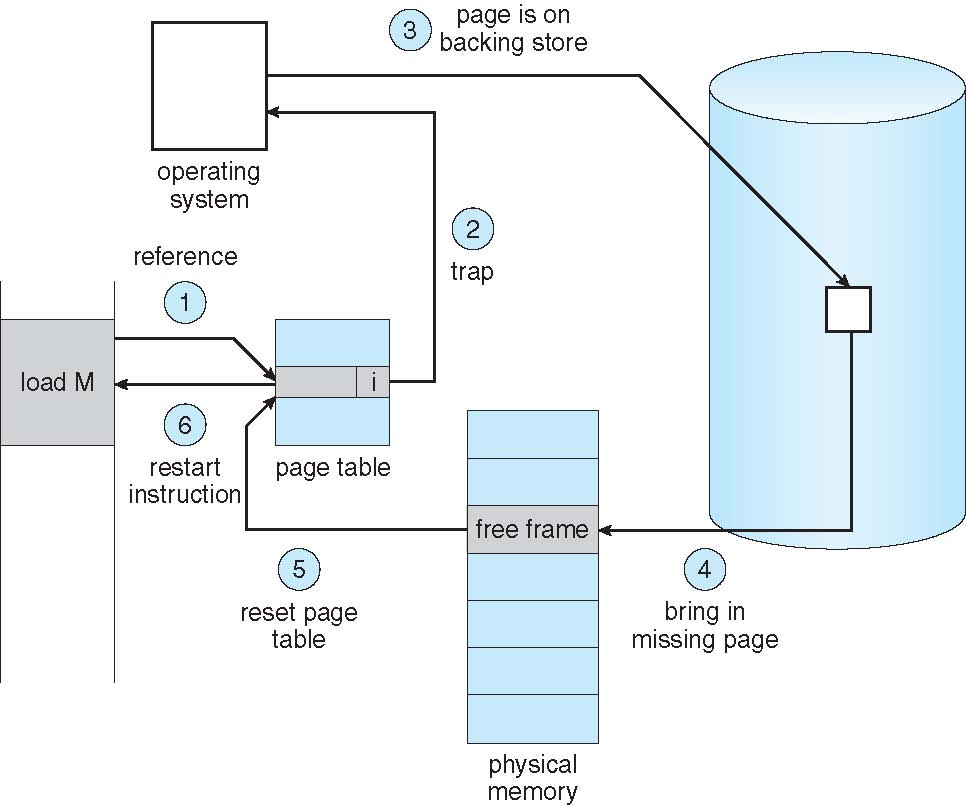
\includegraphics[scale=1]{img/C07_memoria/fallo_pagina.jpg}
\caption{Proceso que ocurre al existir un fallo de página}
\label{fig:fallo_pagina}
\end{figure}

El proceso de \textbf{intercambio} ocurre cuando es detectada una página
inválida y está se encuentra en el disco, pero no hay marco libre en la memoria
principal para ubicarla. Es en este punto donde ocurre lo descrito en la figura
\ref{fig:intercambio}, donde primero se debe llevar a la ``víctima'' desde el
marco en la memoria principal al disco, marcar su página como inválida, luego
llevar la página requerida del disco al marco liberado y marcar esta última
página como ahora válida. Luego se continúa la ejecución con la página cargada
en un marco.

\begin{figure}[htbp]
\centering
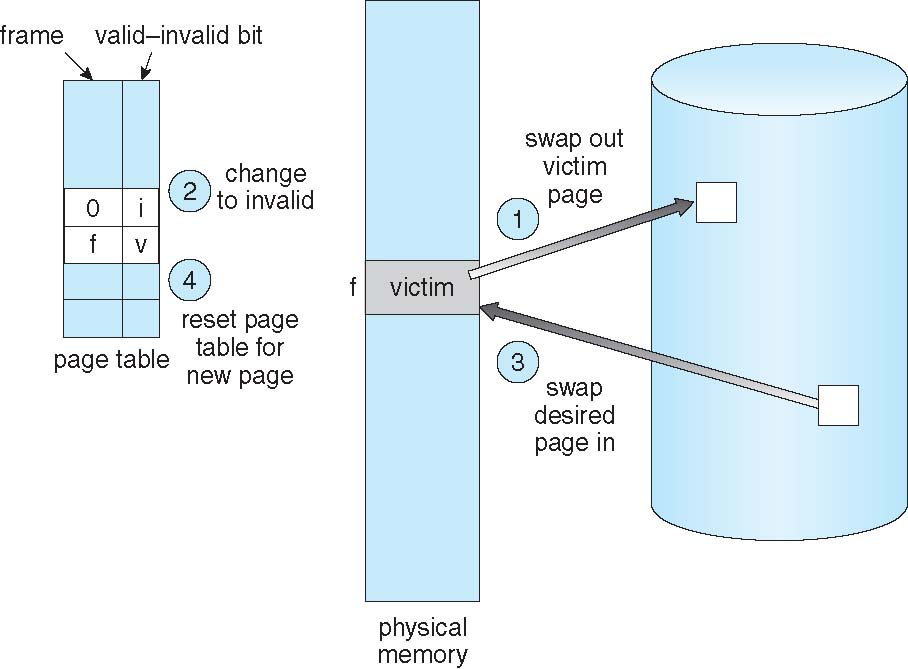
\includegraphics[scale=1]{img/C07_memoria/intercambio.jpg}
\caption{Proceso de intercambio de páginas}
\label{fig:intercambio}
\end{figure}

Un uso lógico de la memoria virtual es cuando el sistema no dispone de más
memoria principal para la creación de nuevos procesos. Adicionalmente el uso de
memoria virtual permitirá disponer en el sistema de un espacio de
direccionamiento virtual mayor al real para los procesos, ya que a pesar de no
tener marcos para todas las páginas del proceso este podría tener aquellas
páginas que no este utilizando en la memoria virtual y solo traerlas a principal
cuando las necesite usar.

\subsection{Algoritmos de reemplazo de páginas}
Para el proceso de intercambio lo crucial es decidir a quién se sacará de la
memoria principal para ser llevado a disco. En estricto rigor se debe determinar
la página que será sacada desde la memoria principal. Para esto existen diversos
algoritmos los cuales serán mencionados a continuación, la idea es encontrar un
algoritmo que en el sistema genere la menor cantidad de fallos de páginas. Lo
último porque el proceso de intercambio es lento ya que implica acceso al
almacenamiento secundario.

En cualquiera de los algoritmos se puede utilizar una optimización que implica
el uso de un \textbf{bit de modificación} (o \textbf{bit dirty}) en la tabla de páginas, este indicará
si la página (que ya esta en disco) fue modificada al estar en la memoria
principal (en un marco). Si fue modificada se copia a la memoria virtual al
existir el intercambio, sin embargo si no fue modificada no se copia, con esto
se reducen los tiempos que dura el fallo de página.

El objetivo de estos algoritmos es ser capaz de elegir una página que será usada
en el futuro más lejano, sin embargo determinar esto es imposible ya que no se
sabe que pasará en el futuro. Sin embargo se puede usar la historia pasada para
poder determinar que páginas podrían usarse en el futuro más lejano. De esta
forma se asumirá, por ejemplo, que una página que no se ha utilizado en el
último minuto no se usará hasta al menos dentro de otro minuto más.

El \textbf{tiempo de acceso efectivo} corresponde al tiempo real que tomará
acceder a la memoria principal si existe un fallo de página. Se define como
$T_{ef} = (1-r) * t_M+r*t_p$, donde:

\begin{itemize}
	\item $t_M$ es el tiempo de acceso a memoria física, por ejemplo 60 ms.
	\item $t_p$ es el tiempo de reemplazo de la página, por ejemplo 12 ms.
	\item $r$ es la tasa de fallos de página.
\end{itemize}

%Si $T_{ef}$ es 10\% superior a $t_M$ se requiere que r = 1 / 2000000.

\subsubsection{Ideal: ``oráculo''}

La estrategia ideal sería consultar el ``oráculo'' y se lleva a disco la página
que permanecerá más tiempo sin ser usada. Lamentablemente esto no se puede
implementar, ya que no se puede ver el futuro. Sin embargo sirve como
referencia.

Ejemplo:
\begin{itemize}
	\item Marcos: 3.
	\item Páginas: 8.
	\item Cadena de referencia: 7,0,1,2,0,3,0,4,2,3,0,3,0,3,2,1,2,0,1,7,0,1
\end{itemize}

¿Cuantos fallos de página generará la cadena de referencia indicada?
% 7, verificar :P

\subsubsection{FIFO}
En este caso se van ubicando las páginas en la memoria en el mismo orden que son
referenciadas, la más ``antigua'' será la que se elegirá como ``víctima'' para
ser sacada en caso de requerir un marco libre. Esta estrategia puede ser
considerada como la peor, sin embargo será las más simple de implementar.

Ejemplo:
\begin{itemize}
	\item Marcos: 3.
	\item Páginas: 8.
	\item Cadena de referencia: 7,0,1,2,0,3,0,4,2,3,0,3,0,3,2,1,2,0,1,7,0,1
\end{itemize}

Luego de la ejecución total del proceso, o sea, cuando se haya procesado toda la
cadena de referencia de páginas habrán ocurrido un total de 15 fallos de
páginas, ver figura \ref{fig:swap_fifo}. Sin embargo la cantidad de fallos de
página dependerá de las solicitudes de páginas, esto significa que con otra
cadena de referencia de memoria podrían haber más o menos fallos de página.

\begin{figure}[htbp]
\centering
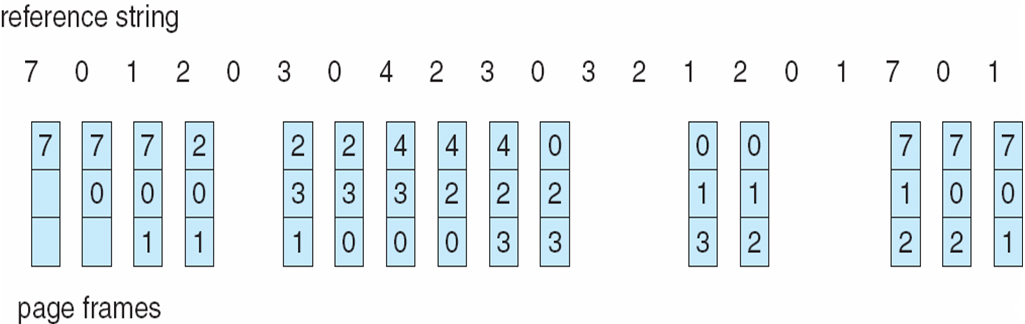
\includegraphics[scale=0.55]{img/C07_memoria/swap_fifo.png}
\caption{Ejemplo de intercambio con algoritmo FIFO}
\label{fig:swap_fifo}
\end{figure}

\subsubsection{LRU}
En este caso la página que es reemplazada es aquella que no ha sido usada en el
último tiempo (\textit{Least Recently Used}), o dicho de otra forma aquella que
fue usada hace más tiempo. Para esto se debe llevar por cada página una
asociación con el tiempo de la última vez que la página fue referenciada.

Implementación:
\begin{enumerate}[a)]
	\item \textbf{Con un contador}: cada entrada de página en la tabla de
páginas tiene un contador, cada vez que la página es referenciada el reloj es
copiado al contador. Cuando una página necesita ser cambiada se mira el contador
y se busca el valor más pequeño. Este método es sencillo de implementar pero
tiene el problema de requerir buscar en toda la tabla de páginas para encontrar
la usada hace mas tiempo, por lo cual resulta muy ineficiente y cara de
implementar. En la práctica no es utilizada.
	\item \textbf{Con una pila}: se mantiene una pila con los números de
página del sistema, cada vez que una página es referenciada se mueve al tope de
la pila. Por lo cual cuando se requiere una página para intercambiar se saca
aquella que esta más abajo en la pila.
\end{enumerate}

\subsubsection{Second chance o estrategia del reloj}
Esta es una aproximación de LRU donde se elige una página que lleve bastante
tiempo sin ser utilizada. Se podría cometer un error y no sacar la que lleve más
tiempo sin ser usada, pero esto es una aproximación que busca aumentar la
velocidad.

El núcleo coloca el bit ``r'' o \textbf{bit de referencia} en 0. Si la página es
referenciada el hardware del procesador (la MMU) coloca el bit ``r'' en 1 cuando
la página se usa. El sobre costo en esto es muy bajo, ya que solo implica ir a
la tabla de página y cambiar un bit. Este cambio se realiza en la TLB, por lo
cual cada cierto tiempo se deberá actualizar el bit en la memoria principal,
pero no es común tener que actualizar de la TLB a la memoria principal.

La página se puede llevar a disco cuando ``r'' permanece en 0 por ``suficiente''
tiempo. ¿Cómo se considera el tiempo? Para esto se utiliza una lista circular
donde cada vez que se quiere sacar una página de la memoria principal se
consulta el bit ``r'', si es 1 la página es dejada en memoria principal (dando
una segunda oportunidad) y su bit es puesto a 0, se continúa así hasta encontrar
una página con su bit de referencia en 0. Se marca el bit de referencia en 1
cada vez que la página es referenciada y se parte revisando a contar de la
página que se cambio la vez anterior.

En la figura \ref{fig:swap_secondchance} se puede apreciar el funcionamiento del
algoritmo, al lado izquierdo desde donde se inicia la búsqueda y al lado derecho
el estado final de los bits de referencia y la ``víctima'' que fue elegida.

\begin{figure}[htbp]
\centering
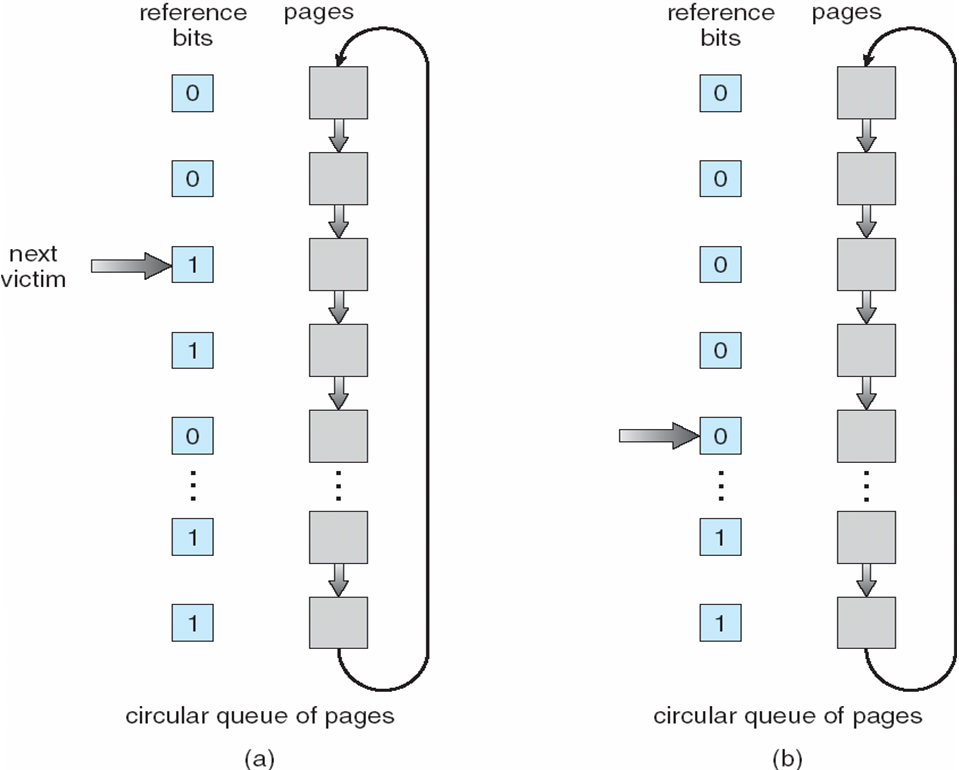
\includegraphics[scale=0.6]{img/C07_memoria/second_chance.png}
\caption{Ejemplo de intercambio con algoritmo Second Chance}
\label{fig:swap_secondchance}
\end{figure}

Esta estrategia es utilizada hoy en día, su seudo código se muestra a continuación:

\begin{verbatim}
while (bitR(cursor())==1) {
  bitR(cursor()) = 0
  avanzarCursor()
}
reemplazarCursor()
AvanzarCursor
\end{verbatim}

Si todas las páginas tienen su bit de referencia \textit{r} en 1 se deberá dar la vuelta completa poniendo los bits en 0 hasta volver a la primera página revisada la cual ahora tendrá el bit en 0 y se escogerá. Esto es una situación anómala ya que en estricto rigor no se está determinando lo esperado, ya que todas estaban en iguales condiciones y se terminó sacando la primera consultada. Se da cuando el tiempo en que se demora en dar la vuelta a la lista es muy grande, sin embargo en la práctica es muy poco probable que ocurra y no es considerado como un problema real.

Un problema real es el \textbf{thrashing}, que corresponde a la situación cuando la tasa de fallos de páginas es muy alta. Esto ocurre cuando ocurren fallos de páginas muy seguidos, el cursor avanza muy rápido y los discos al ser lentos (tiempo de acceso alrededor de 10 ms) se podrían atender aproximadamente 100 fallos de página por segundo. En esta situación el sistema operativo trabajará llevando procesos de disco a RAM y de RAM a disco, pero no se hará trabajo útil. La CPU pasa el 99\% del tiempo ociosa y el disco de \textit{paging} pasa el 100\% del tiempo ocupado, lo anterior significa que los procesos no avanzan. Recuperarse de esto es muy complicado de forma automática, por lo cual la solución es matar procesos, lo cual no se hace automáticamente. El problema de hacerlo manualmente es que se requiere memoria para conectarse al equipo, luego memoria para ver los procesos y matar alguno que ocupa mucha RAM. Caso extremo, la solución es reiniciar.

\subsubsection{Estrategia del \textit{working set}}

La idea de este método es utilizar la combinación de paginamiento por demanda con \textit{swapping}, basado en un \textit{working set} por proceso evitando el \textit{thrashing}.

El \textit{working set} son las páginas que ha usado recientemente el proceso. La estrategia del reloj no hace una distinción por proceso, compara todas las páginas de los procesos juntas. En este caso el tiempo considerado para correr el reloj es solo cuando el proceso está avanzando o sea el tiempo virtual del proceso.

Más formalmente, $WS_P(t, \Delta t)$ es el conjunto de páginas usadas por $P$ en el intervalo $(t-\Delta t, t)$ de tiempo virtual. Se debe mantener el $WS$ de cada proceso actualizado en memoria, para esto se calcula el $WS$ para cada proceso cada $\Delta t$ unidades de tiempo virtual. Aquellas páginas que no pertenecen al WS se pueden llevar a disco.

La principal desventaja de este método es que siempre se debe estar calculando el \textit{working set}, a pesar de que haya mucha memoria física disponible. En el caso de Linux, cuando la CPU no tiene ``nada'' que hacer, el núcleo se pone a actualizar tablas para la estrategia del reloj.

Para el cálculo del $WS_P$, que se realiza cada $\Delta t$ segundos de uso de CPU (tiempo virtual), tenemos $C$ como el conjunto de páginas candidatas para ir a disco. Con este $C$ se define la forma de realizar el $WS_P$ según el siguiente algoritmo:

\begin{verbatim}
WSp = vacío
para toda página q perteneciente a P residentes en memoria física {
  if(bitR(q)==1) {       // si el bit r es 1
    WSp = WSp U {q}      // se agrega la página q al WS
    bitR(q) = 0          // se pone el bit r en 0 (para quitarla a futuro)
  } else {
    C = C U {q}          // si el bit r era 0 se agrega al conjunto C
  }
}
\end{verbatim}

Cuando se deba elegir una página para llevar a disco bastará recorrer el conjunto de páginas $C$ y revisar su bit de referencia \textit{r} (que podría haber sido modificado en el $\Delta t$).

Cuando ocurre un fallo de página se debe seleccionar una página para intercambiar, esto se puede realizar con el siguiente algoritmo:

\begin{verbatim}
while C no esté vacío {  // mientras vayan quedando elementos en C
  Sea q e C              // por cada elemento q perteneciente a C
  C = C \ {q}            // quitar q del conjunto C
  if(bitR(q)==0) {       // si el bit de referencia es 0
    return q             // se retorna q para reemplazar
  }
  WSp = WSp U {q}        // si el bit r estaba en 1 se coloca a q en el WS
}
Swap()                   // se cambia la página q por la requerida
\end{verbatim}

Cuando la sumatoria de los \textit{working set} de cada proceso, $\sum_{i=1}^{n} {WS_{P_i}}$, es mayor a la memoria física disponible se debe empezar a hacer intercambio de procesos completos. Un proceso no puede correr eficientemente si su \textit{working set} es más grande que la memoria física del computador.

Para el caso del sobre costo en los fallos de páginas definamos:

\begin{itemize}
	\item \textit{pf}: fallos de página.
	\item \textit{ta}: tiempo de acceso al disco
	\item \textit{tt}: tiempo total que tomaron los fallos de página
\end{itemize}

Para determinar el tiempo total se utilizará: $pf * ta = tt$, si consideramos un proceso que causa 10 fallos de página en un segundo de uso de CPU, en este caso el sobre costo sería $10 * 10 = 100$. Estos 100 ms representan un 10\% de sobre costo sobre el segundo de CPU utilizado.

\section{Ejercicios y preguntas}
\begin{enumerate}
	\item ¿Cuál es la forma más simple de asignar memoria principal?.
	\item Describa los conceptos: base, límite y desplazamiento, y como están relacionados.
	\item ¿Qué es un \textit{segmentation fault}?.
	\item ¿Qué implica asignar la memoria de forma contigua?.
	\item Explique los tres tiempos en que puede ser realizado el enlace de direcciones.
	\item ¿Cuál es el inconveniente de utilizar intercambio con los enlaces en tiempo de compilación o en tiempo de carga?, explique.
	\item ¿Cuál es la relación entre direcciones virtuales y físicas?.
	\item ¿Las direcciones virtuales son contiguas?.
	\item ¿Qué ventajas presenta el uso de direcciones virtuales?.
	\item ¿Por qué no era posible instalar Unix en los ordenadores con procesadores 8088?.
	\item Fundamente la siguiente premisa: la asignación no contigua de memoria física no implica asignación no contigua de direcciones virtuales.
	\item ¿Cómo se divide el proceso al utilizar segmentación?.
	\item ¿Cuántos segmentos como mínimo se deben asignar al inicio del proceso?.
	\item ¿Cuál es la funcionalidad de la tabla de segmentos?.
	\item Explique el proceso de traducción de dirección virtual a dirección física en un esquema con segmentación.
	\item Cuando un proceso esta en estado inicial, ¿qué método de asignación de segmentos (First-Fit, Best-Fit o Worse-Fit) se utiliza para asignar el segmento de sistema?.
	\item Explique en que consiste la fragmentación externa, como se soluciona.
	\item ¿Cuál es el problema de la compactación?.
	\item Cuando un segmento necesita crecer, explique las dos situaciones que pueden ocurrir.
	\item Fundamente la siguiente premisa: el segmento de código puede ser compartido entre proceso hijos.
	\item ¿Por qué el usar \textit{copy on write} se considera una optimización en la creación de páginas al hacer \texttt{fork}?.
	\item ¿Cuál es la principal diferencia entre segmentación y paginación?.
	\item Los tamaños de las páginas y marcos, ¿son iguales o diferentes?, fundamente.
	\item La cantidad de páginas y marcos, ¿son iguales o diferentes?, fundamente.
	\item Explique el problema de fragmentación interna en las páginas.
	\item Explique el concepto de carga dinámica de páginas.
	\item ¿Qué ventaja tiene el enlace dinámico de bibliotecas?.
	\item Explique el proceso de traducción de dirección virtual a dirección física en un esquema con paginación.
	\item ¿Qué indica el bit de validez (o invalidez)?.
	\item Explique en que consiste y como se maneja un fallo de página.
	\item Explique cuando ocurre el proceso de intercambio.
	\item Explique el proceso de intercambio.
	\item Explique los tres algoritmos de reemplazo de páginas.
\end{enumerate}

\section{Referencias}
\begin{itemize}
	\item Sistemas Operativos, Segunda Edición, Andrew Tanenbaum, Capítulo 4.
	\item Sistemas Operativos, Quinta Edición, Abraham Silberschatz y Peter Baer Galvin, Capítulo 8 y 9.
	\item Sistemas Operativos, Segunda Edición, William Stallings, Capítulo 6 y 7.
\end{itemize}
